\section{Related Work}
Voice assistants such as Amazon Alexa \cite{alexaAssitant}, Google Assistant \cite{googleAssistant}, Apple Siri \cite{siriAssistant}, Microsoft Cortana \cite{cortanaAssistant} and Baidu DuerOS \cite{baiduAssistant} currently dominate the market and are in figure \ref{fig:sprachassistenten} shown. Voice assistants handle the input data of the users differently. Privacy policy of the providers doesn't clearly define, what happens in detail with the input data of a user. In the following, privacy policies of each provider are briefly described.

\begin{figure}[h!]
	\centering
	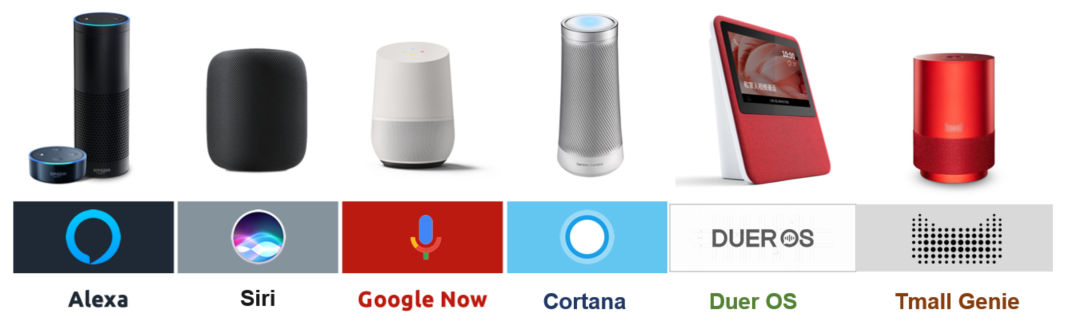
\includegraphics[width=1\linewidth]{Picture/Sprachassistenten}
	\caption[Voice Assistants on the Market\cite{homeVoiceAssistants}]{Voice Assistants on the Market\cite{homeVoiceAssistants}}
	\label{fig:sprachassistenten}
\end{figure}

Amazon Alexa uses the users input to improve the speech services and display personalized advertising. Restricting the use of data for different areas is possible, but this also limits the functionality \cite{alexaPrivacy}.

Google Assistant uses the same permissions that apply to the provider's mobile app \cite{googleShare}. A different attitude to the mobile app is not possible. The interaction with Google Assistant can be used for personalized advertising, like other searches \cite{googlePrivacy}.

To improve pronunciation and functionality, data such as name, contacts, music, search activities and other information is encrypted. The data is not used with the Apple ID but with a randomly generated identifier. This ensures privacy for users \cite{siriPrivacy}.

In the privacy terms of Microsoft's Cortana, it is informed that certain data is "[...] such as searches, calendars, contacts, and places. [...]"\cite{cortanaAssistant} are saved. The data usage of Cortana as Personal Assistant is configurable. If the personalized information is disabled, Cortana can only be used for applications such as searching and scheduling a timer. Cortana does not use personal information for personalized advertising.

Baidu DuerOS also collects user data to improve the voice assistant's speech processing. Qi Lu refers to the many scenarios in which Baidu collects data, with which Baidu is to make the leap to the top of the world in artificial intelligence. The personal data of a user are transmitted. Baidu does not offer configurable privacy \cite{baiduAI}.

Since February there is the voice assistant Mycroft Mark II on the market, which is combining openness and privacy \cite{mycroftsmartspeaker}. The functionalities are limited here, since the language assistant stores no data to further train and understand the user context.